\section{Results}
The output wave-forms as seen on the oscilloscope for different values of loads and capacitance are shown here in Figs 5 to 9.
\begin{figure}[H]
    \centering
    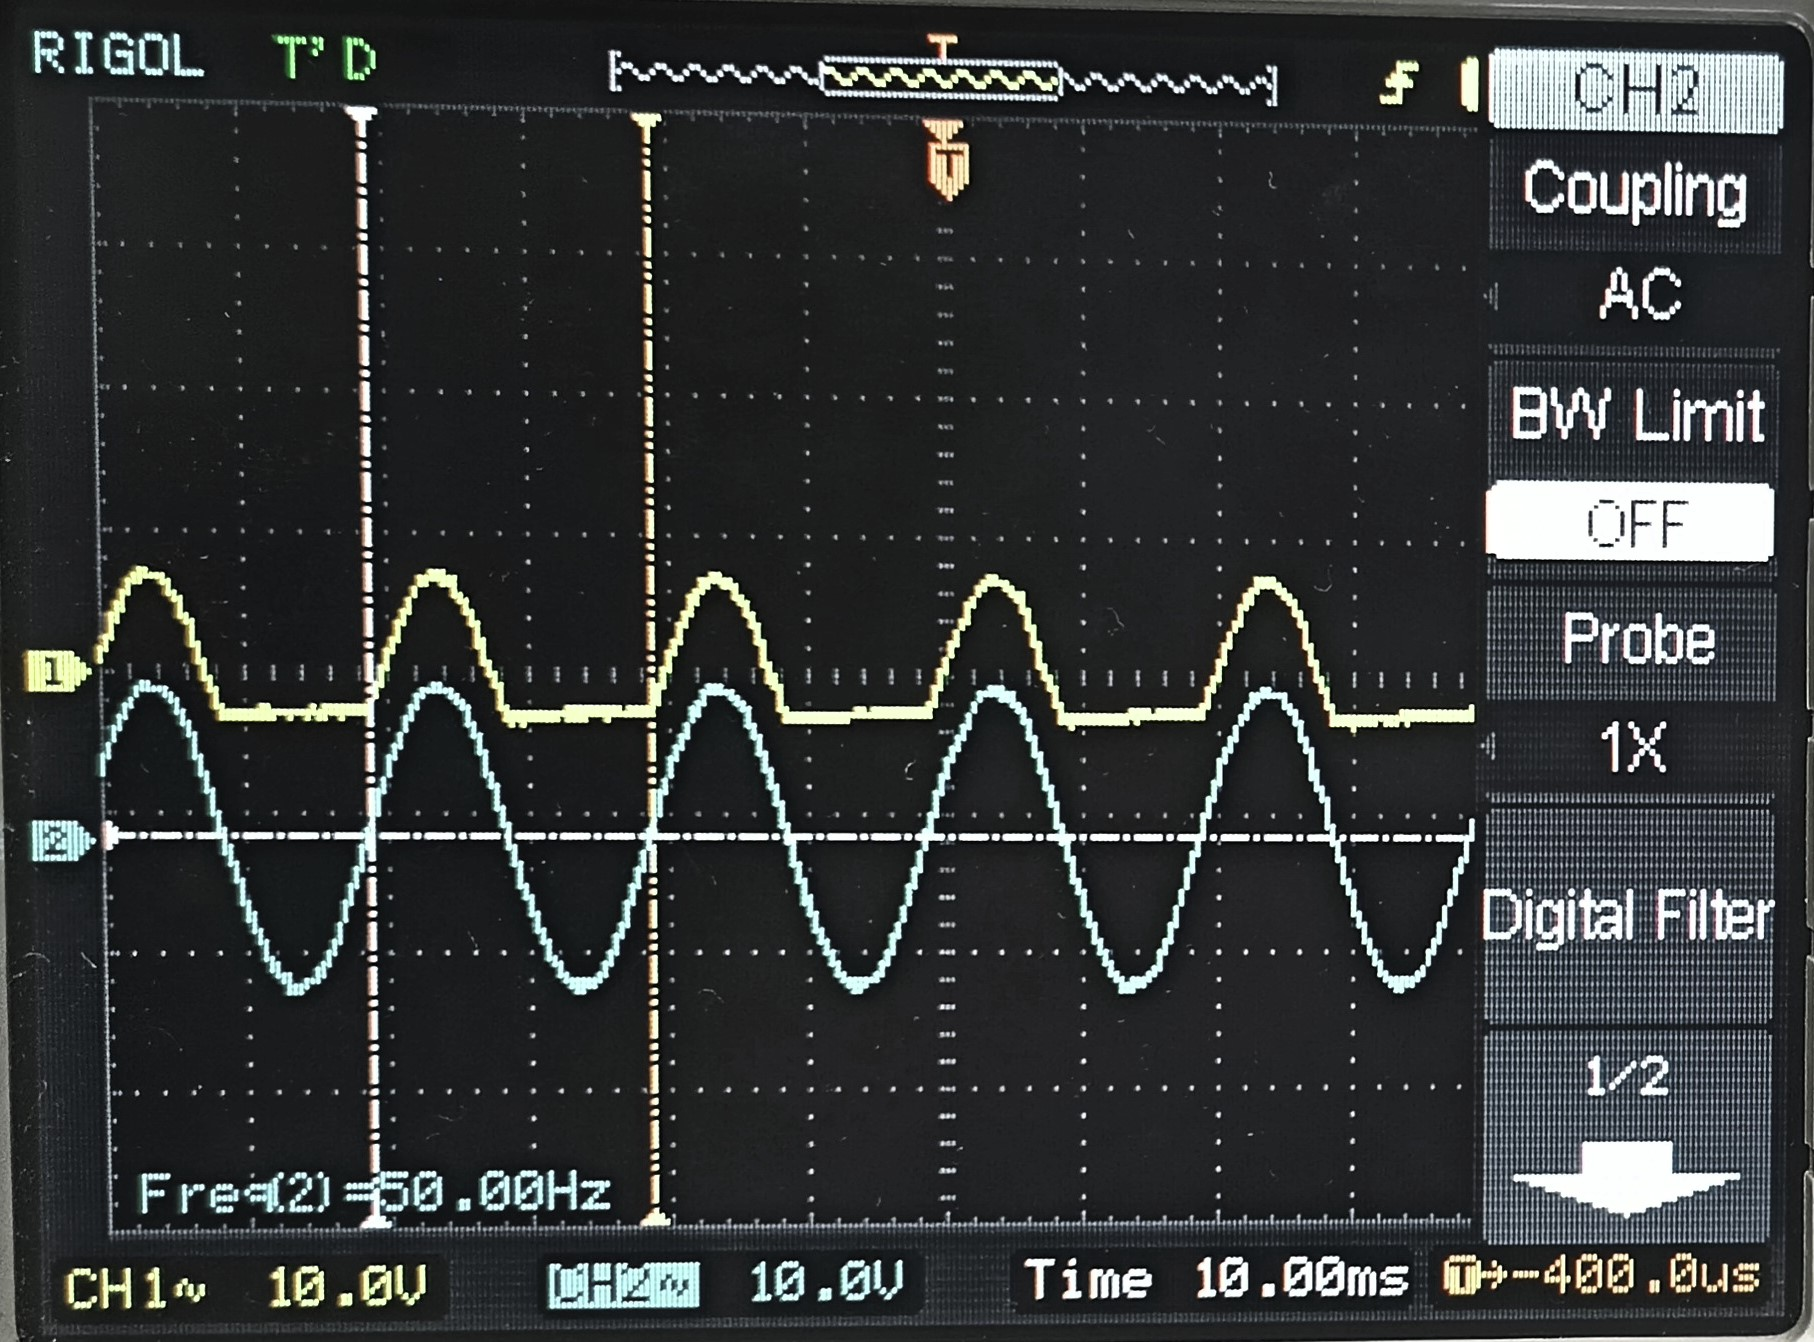
\includegraphics[width=0.72\columnwidth]{images/00.jpg}
    \caption{Half wave rectifier without a filter at $R = 2.2k\Omega$}
\end{figure}

\begin{figure}[H]
    \centering
    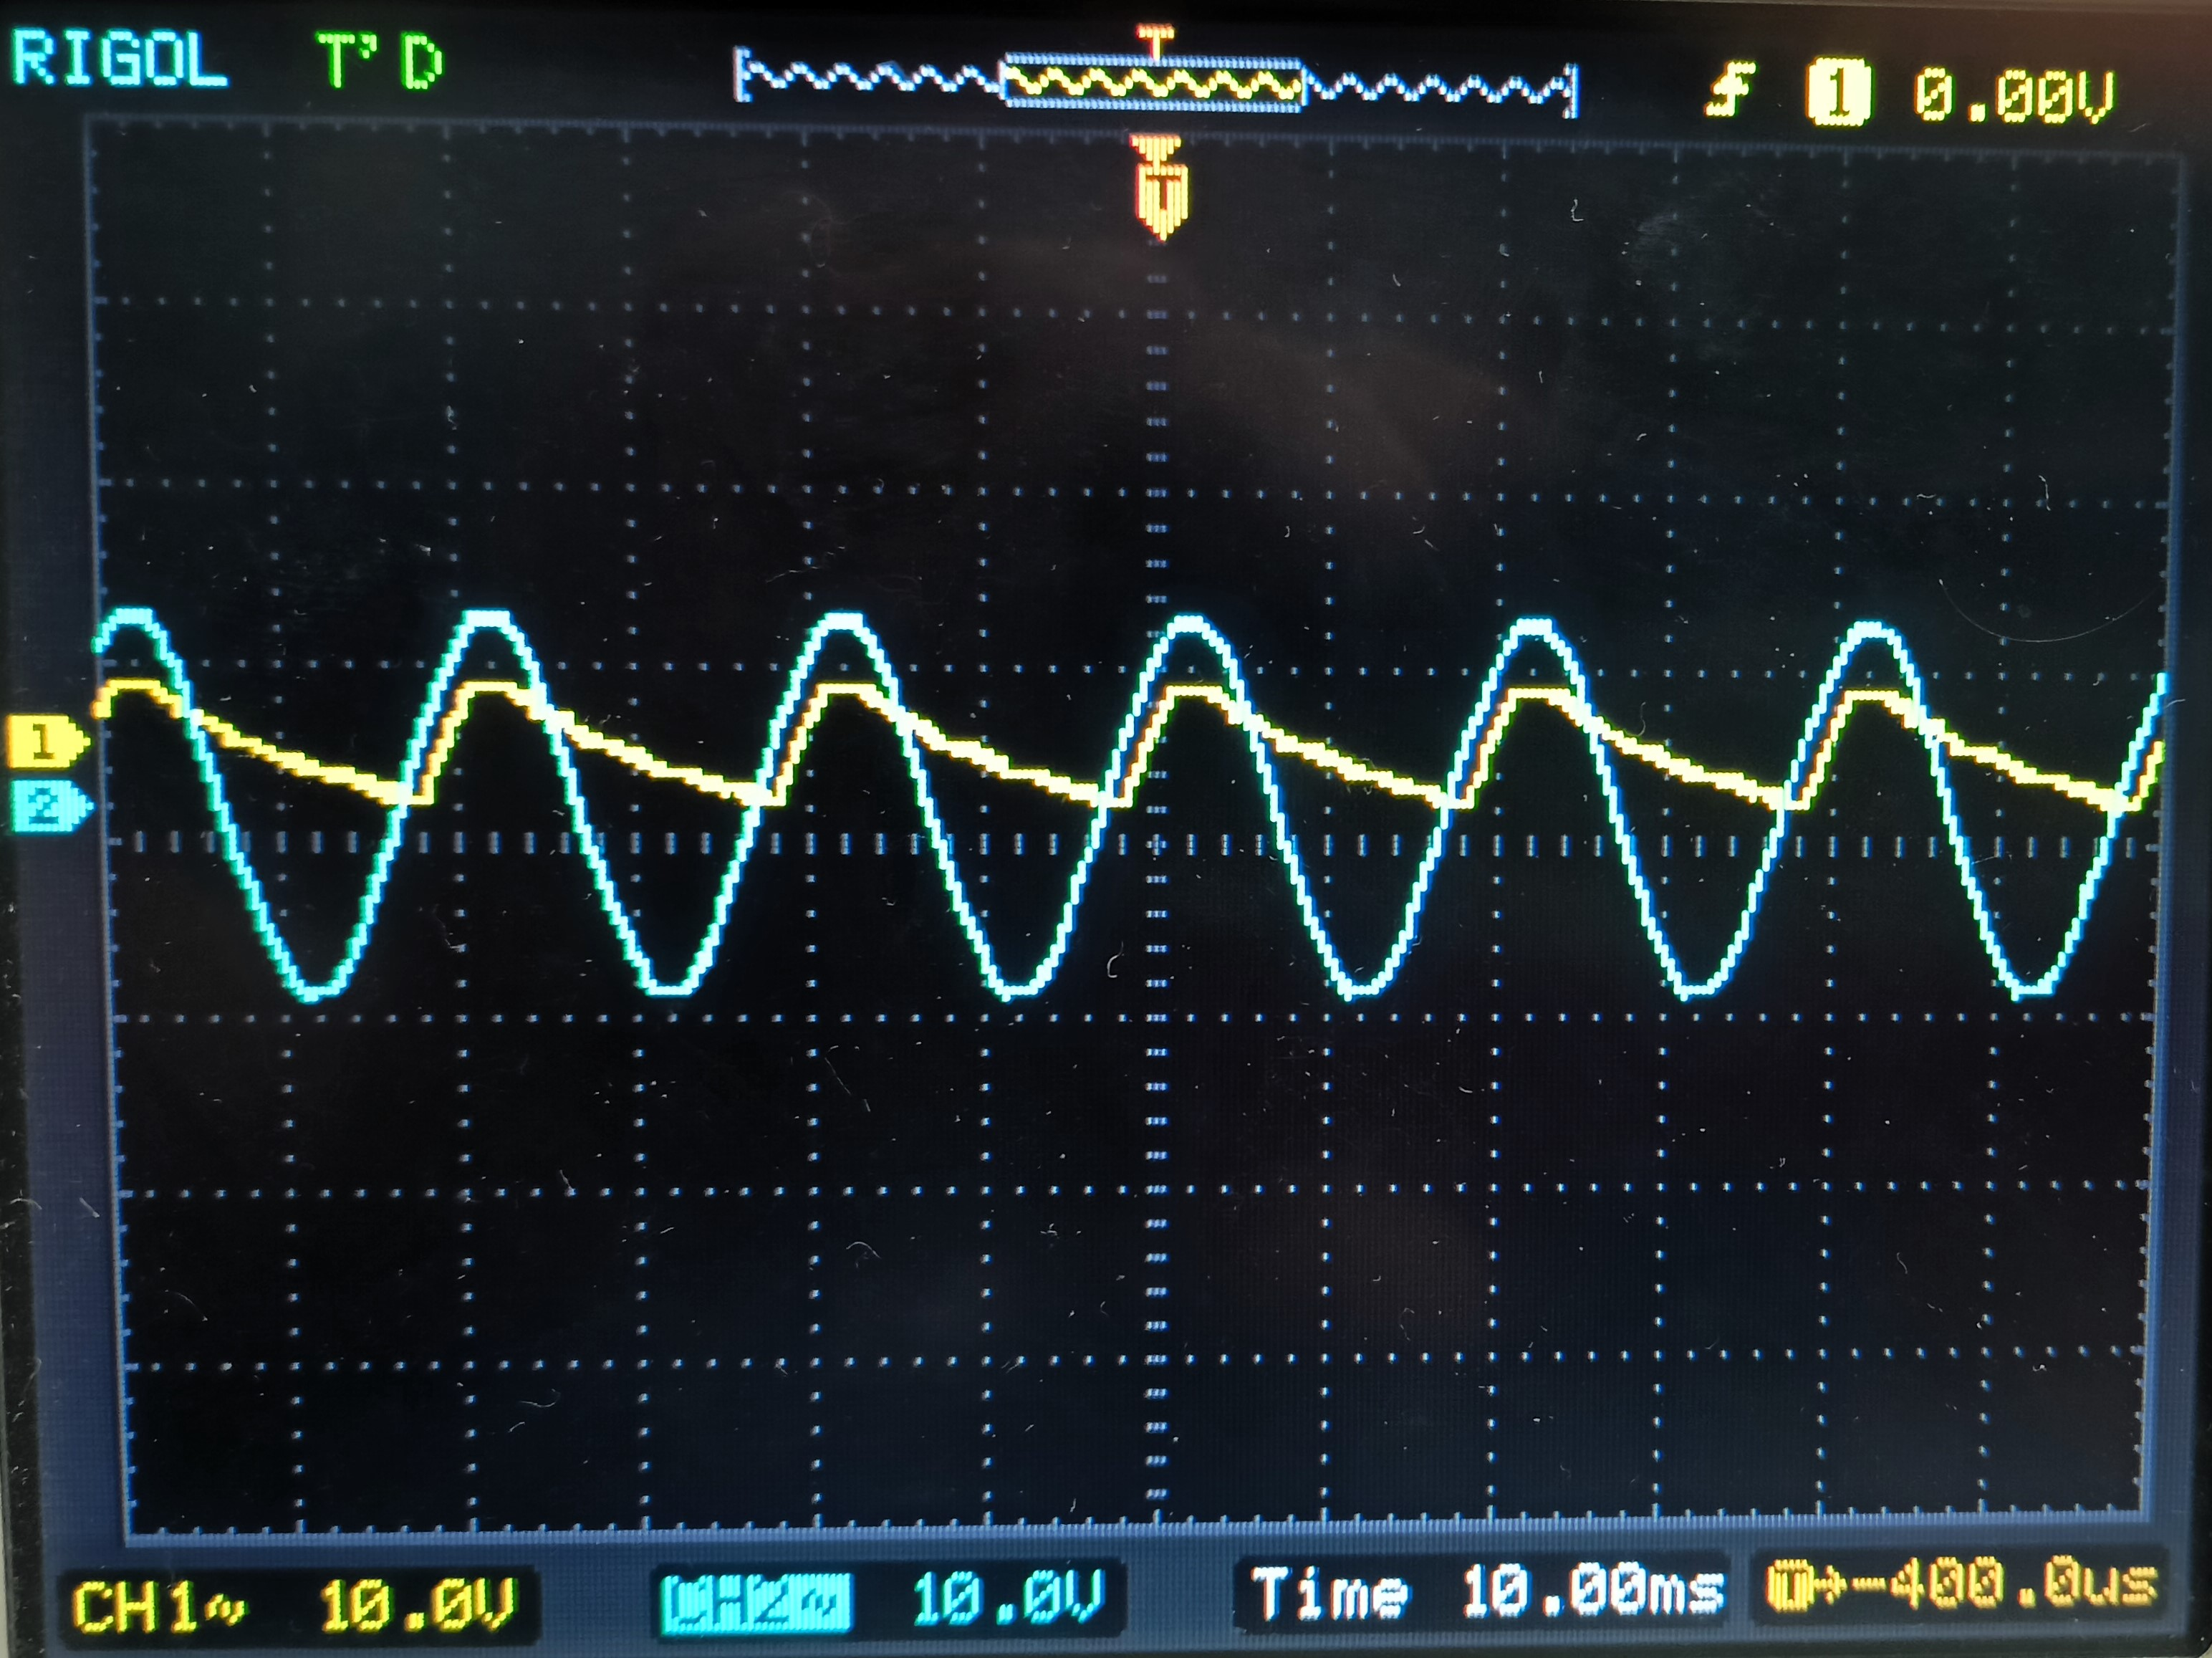
\includegraphics[width=0.72\columnwidth]{images/11.jpg}
    \caption{Half wave rectifier with a filter at $R = 1.5k\Omega$ and $C = 10.71\mu F$}
\end{figure}

\begin{figure}[H]
    \centering
    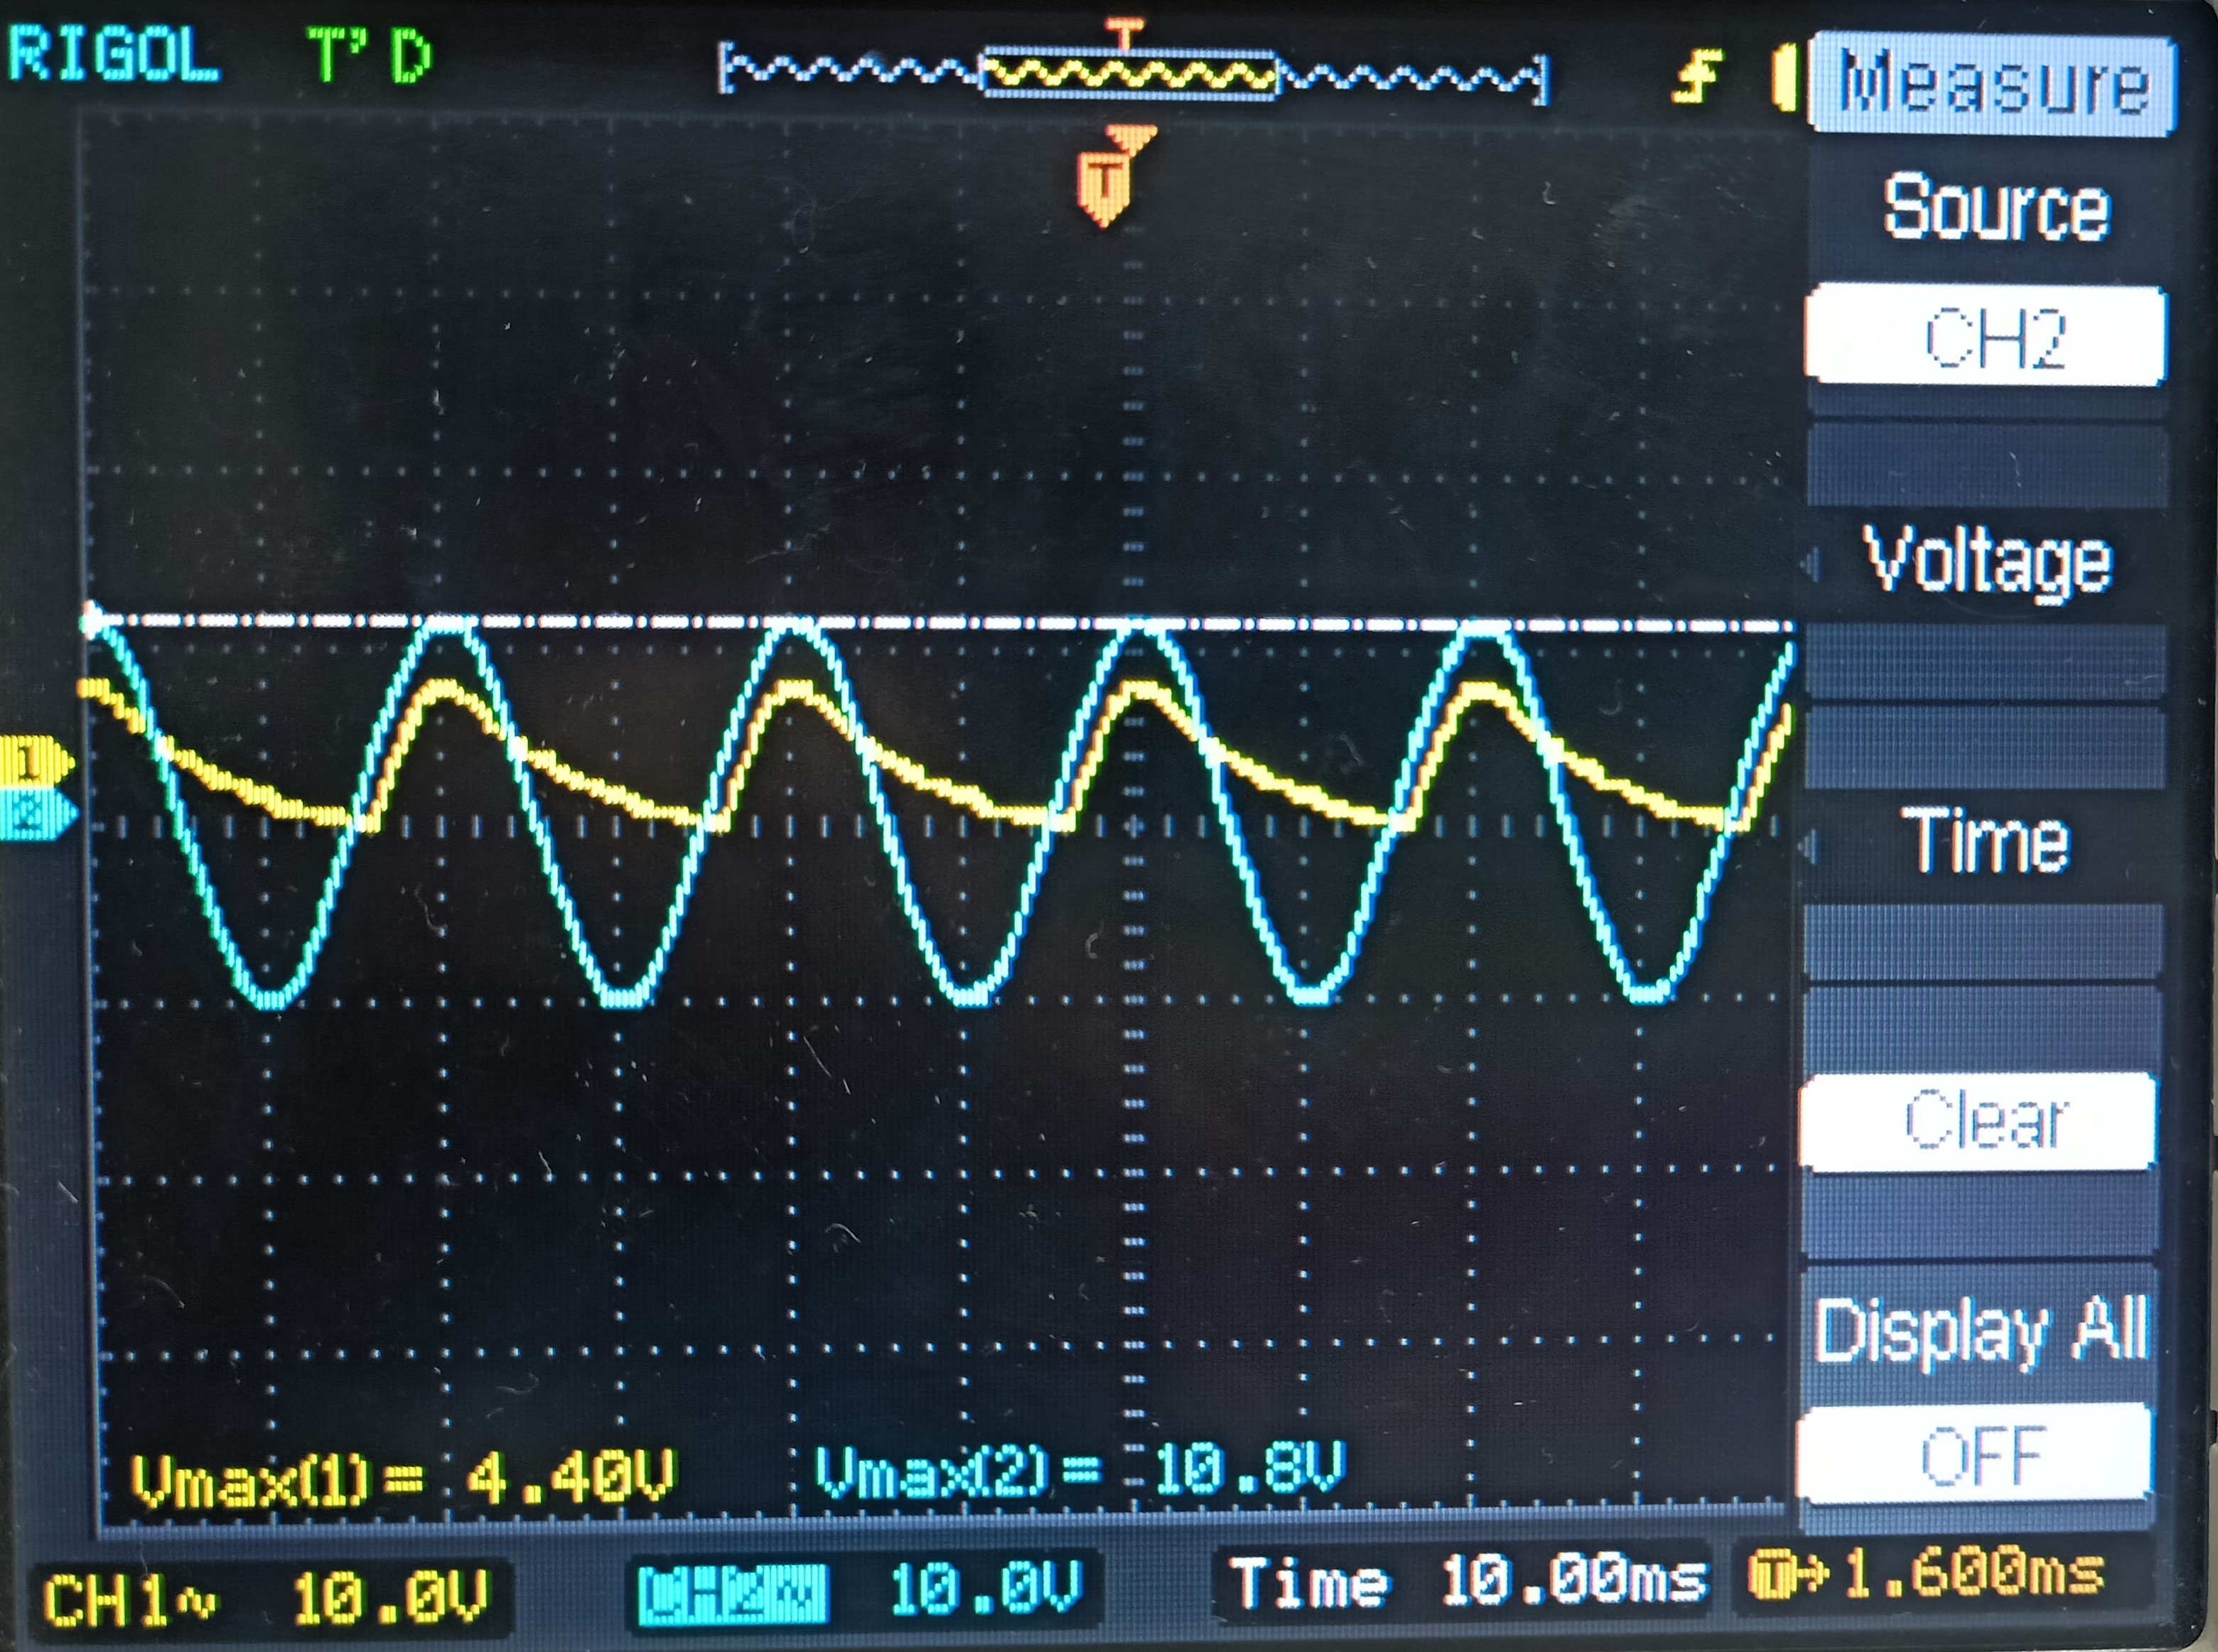
\includegraphics[width=0.72\columnwidth]{images/21.jpg}
    \caption{Half wave rectifier with a filter at $R = 1.0k\Omega$ and $C = 28.83\mu F$}
\end{figure}

\begin{figure}[H]
    \centering
    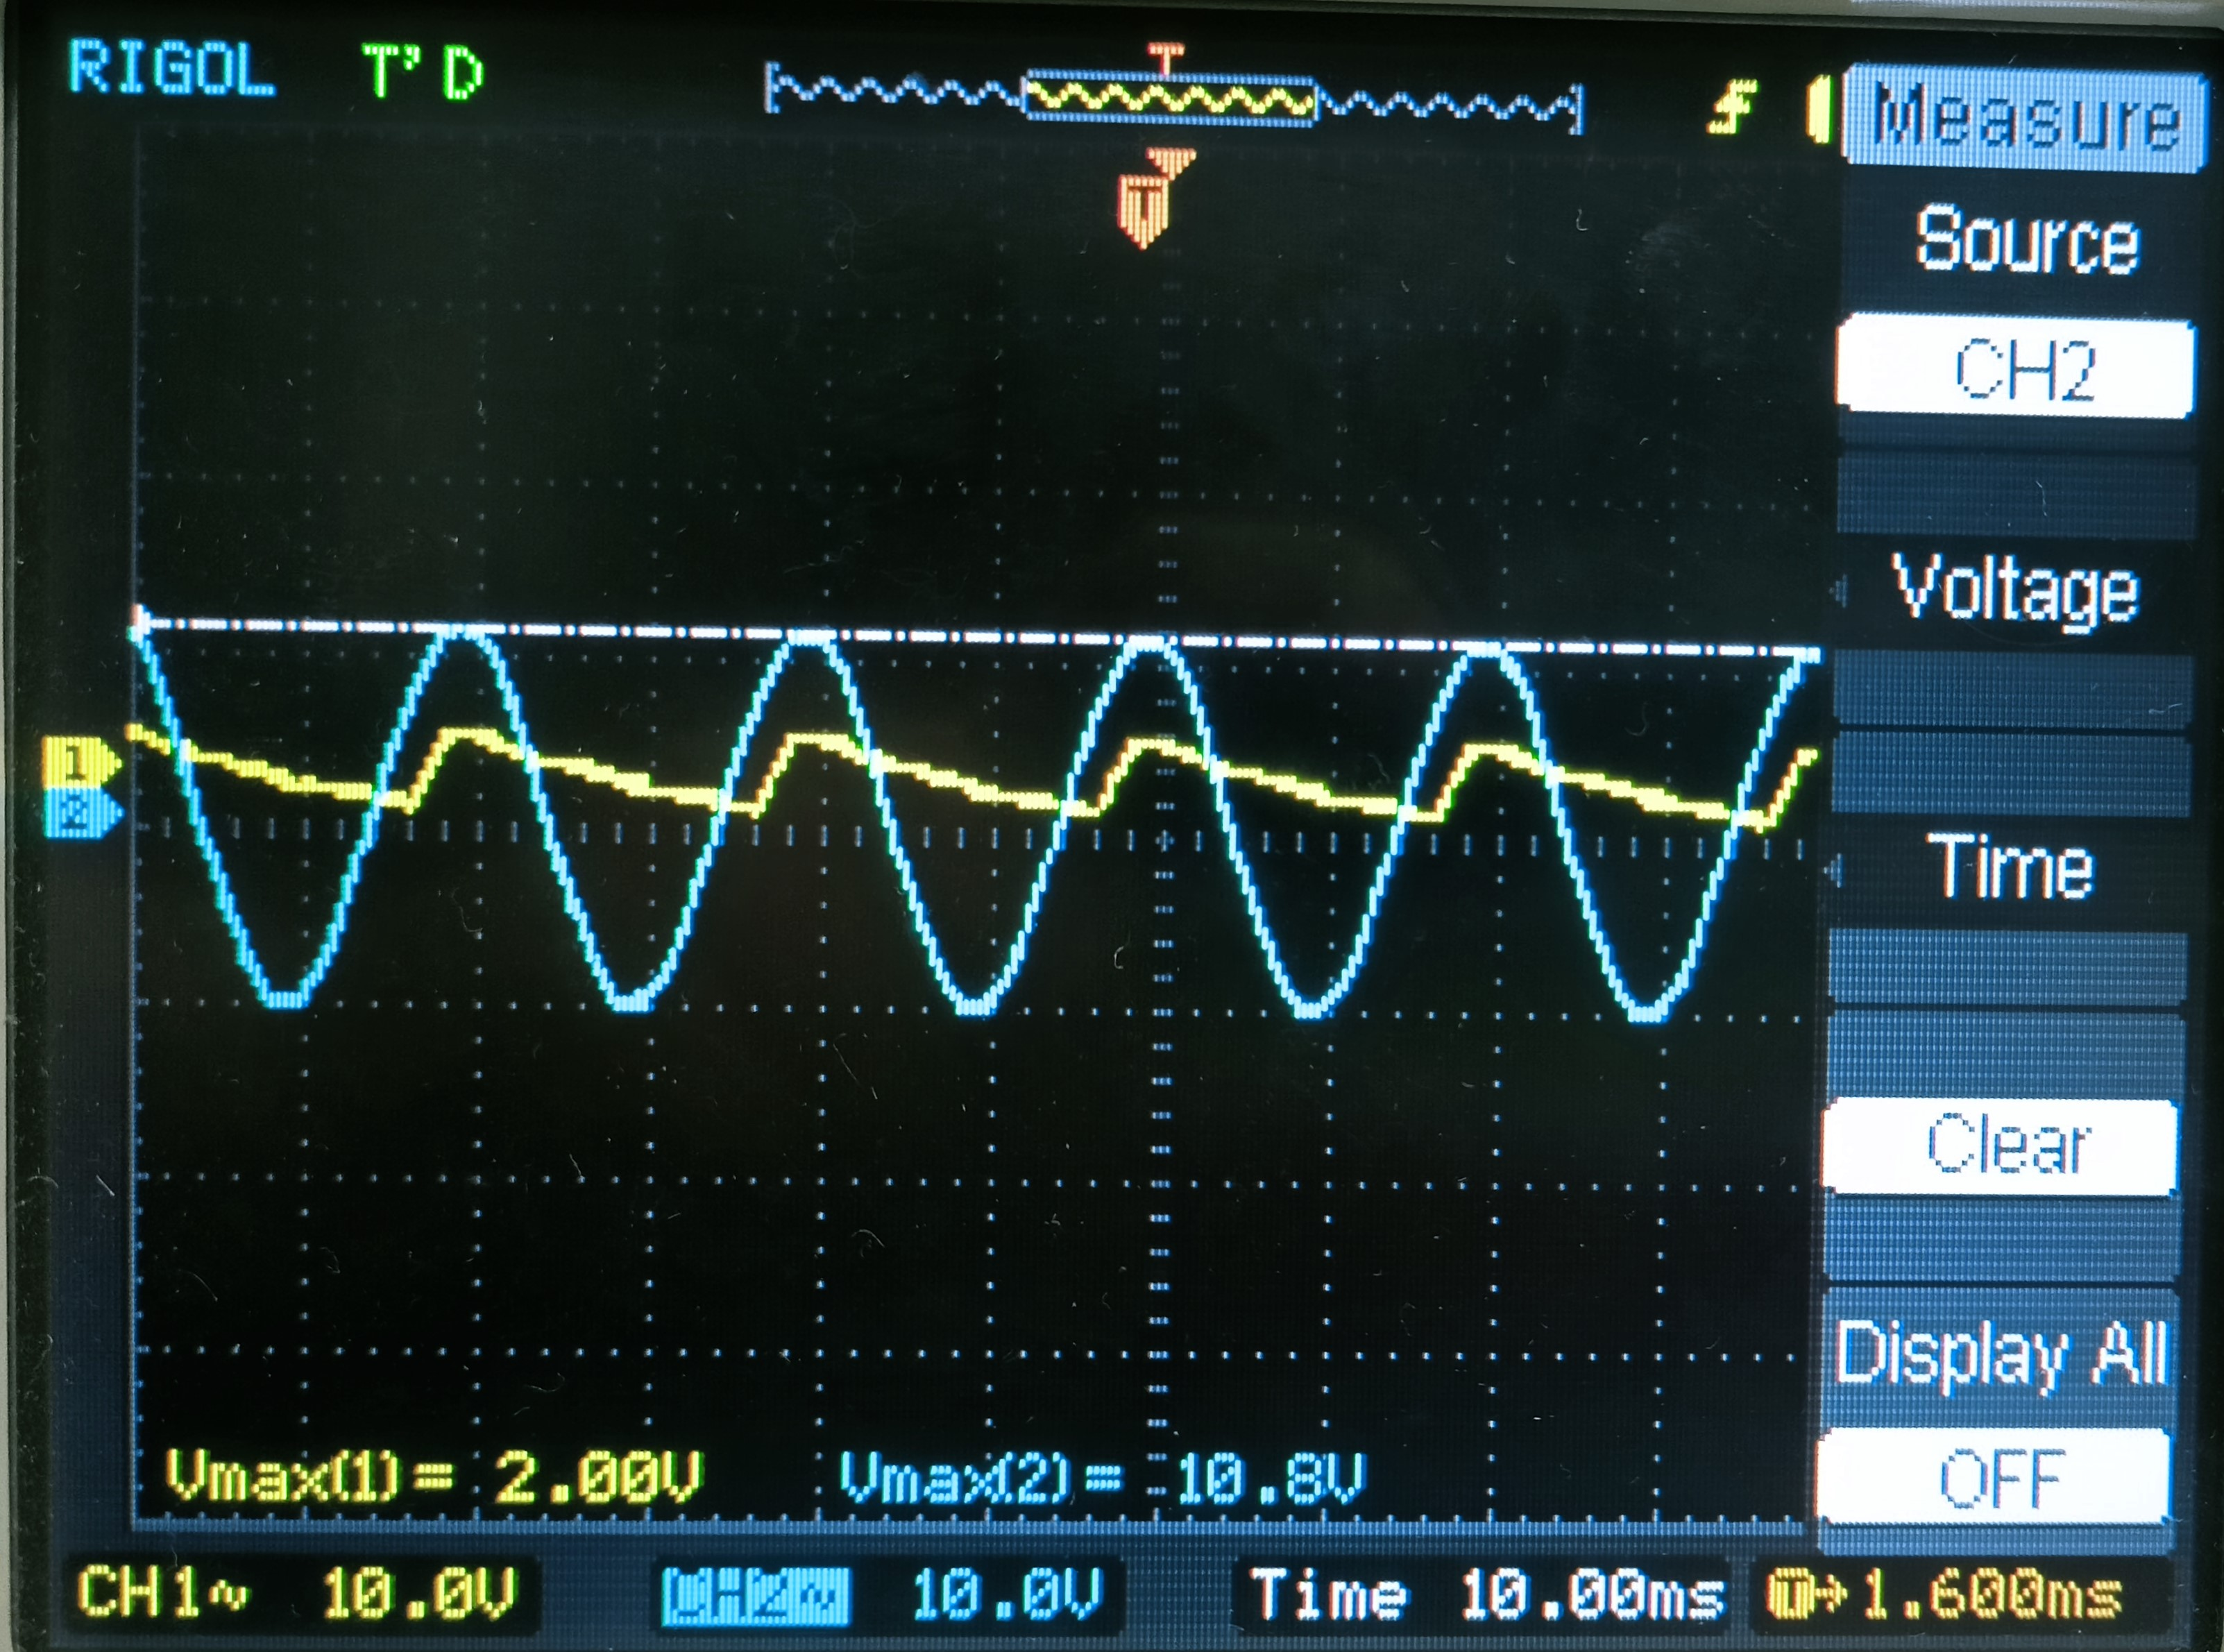
\includegraphics[width=0.72\columnwidth]{images/31.jpg}
    \caption{Half wave rectifier with a filter at $R =1.5k\Omega$ and $C = 23.50\mu F$}\end{figure}

\begin{figure}[H]
    \centering
    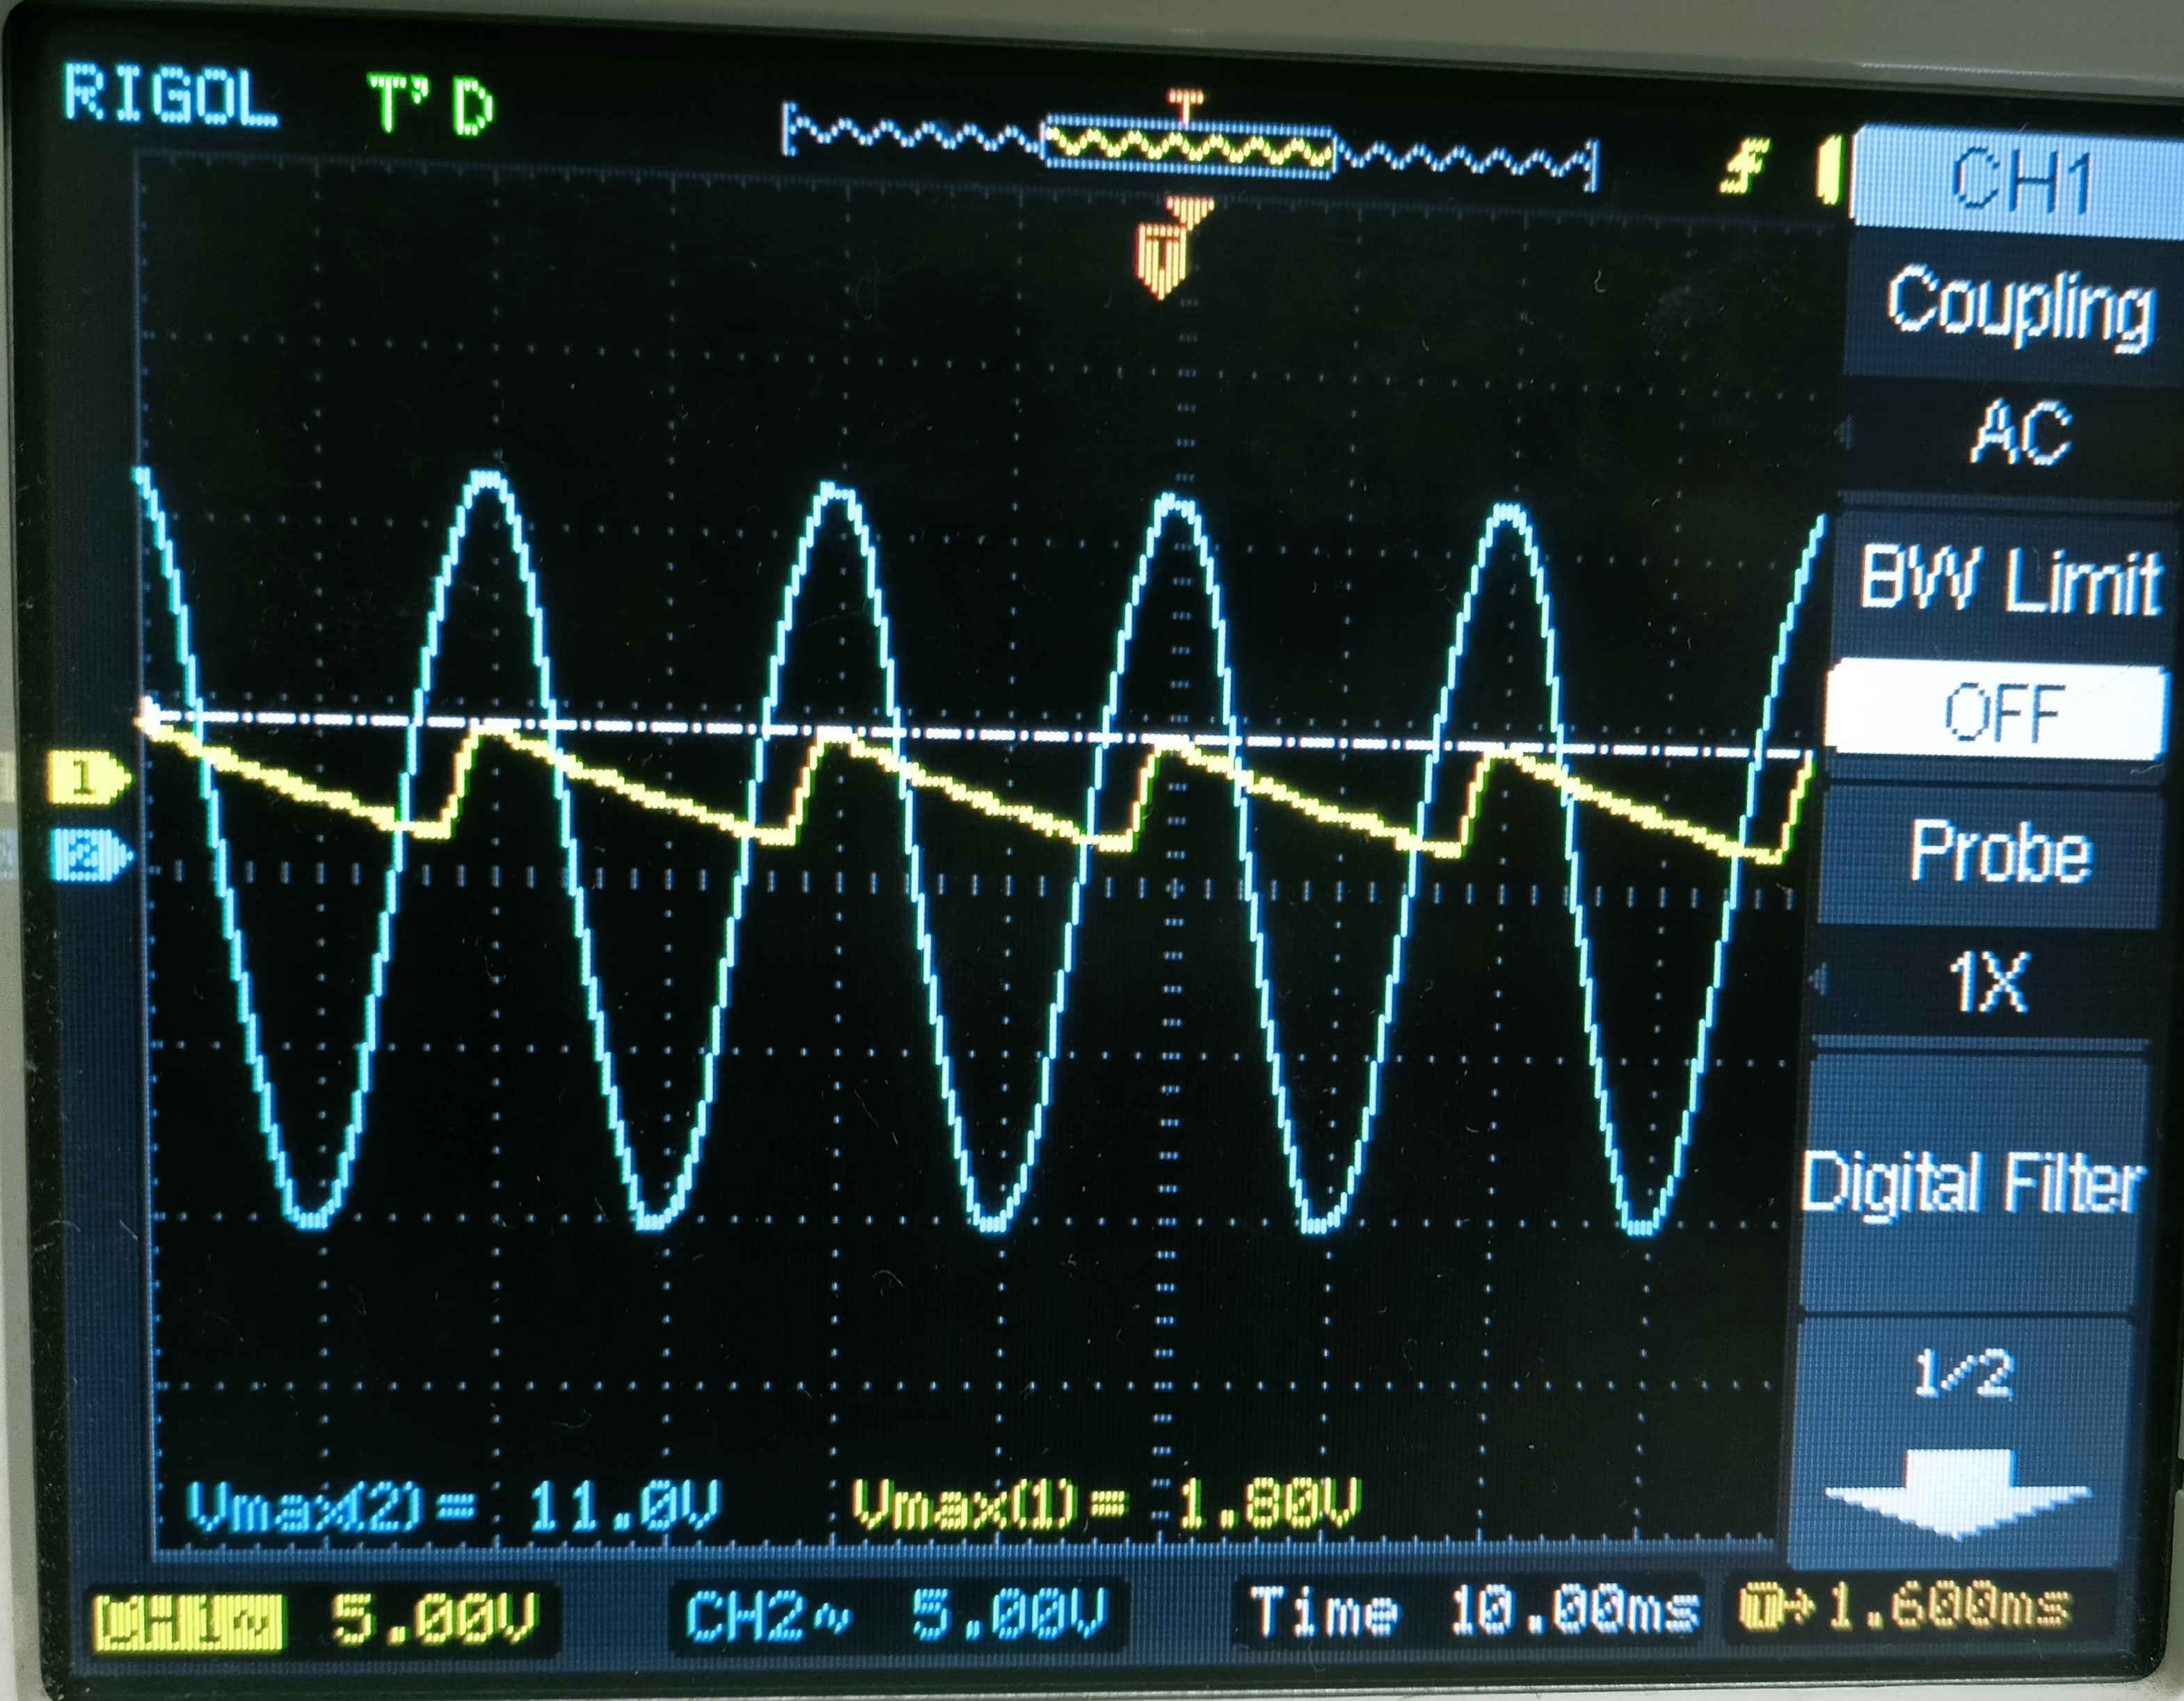
\includegraphics[width=0.72\columnwidth]{images/33.jpg}
    \caption{Half wave rectifier with a filter at $R = 2.2k\Omega$ and $C =23.50 \mu F$}
\end{figure}

\section{Conclusion}
For the half-wave rectifier circuit without the filter, we can see that the ripple factor and rectification efficiency stays around the same for different loads with an average value,

\begin{align*}
    r &= 1.23\\
    \eta &= 32.85\%
\end{align*}

where $r$ is close to the theoretically calculated value and the rectification efficiency is less than the ideal value, as predictable.

For the half-wave rectifier circuit with the filter, we can see that for a particular capacitance, $r$ is inversely proportional to the load resistance. Similarly, for a particular load resistance, $r$ is inversely proportional to capacitance. The lowest $r$ measured is 0.073.

Since we are ideally aiming for the lowest ripple factor in the output signal (i.e. maximise the DC component), we can conclude that a proper combination of optimally large values of RC will give us a steady output signal.

\section{Precautions}
\begin{enumerate}
    \item The transformer must be handled carefully.
    \item Switch on the circuit only after verifying the connections to be proper.
    \item Visualise the output on the oscilloscope to make sure the rectification is happening before taking readings.
    \item Do not change the resistor or the capacitor while the circuit is switched on.
\end{enumerate}